\documentclass{beamer}
%% Possible paper sizes: a0, a0b, a1, a2, a3, a4.
%% Possible orientations: portrait, landscape
%% Font sizes can be changed using the scale option.
\usepackage[portrait,size=a1,scale=1.4]{beamerposter}
\usetheme{LLT-poster}
 \usecolortheme{ComingClean}
%\usecolortheme{Entrepreneur}
% \usecolortheme{ConspiciousCreep}  %% VERY garish.
\usepackage{gensymb}
\usepackage[utf8]{inputenc}
\usepackage[T1]{fontenc}
\usepackage{libertine}
\usepackage[scaled=0.92]{inconsolata}
\usepackage[libertine]{newtxmath}

\usepackage{mwe}

\author[p.duernay@protonmail.com]{Philipp Duernay}
\title{Gate Detection for Autonomous MAV Race}
\institute{TU Delft}
% Optional foot image
\footimage{		
\includegraphics[height=3cm]{fig/tudelft}  
\includegraphics[height=3cm]{fig/mavlab} 
	
\includegraphics[height=3cm]{fig/prgroup}}

\begin{document}
\begin{frame}[fragile]
\begin{columns}[T]

%%%% First Column
\begin{column}{.25\textwidth}

	
\begin{block}{Overview}
This thesis investigates the development of a vision based navigation system to be applied in autonomous drone racing, in particular the race at IROS 2018 in Madrid. The race court consists of several gates that need to be passed one after another. The image is recorded from a monocular camera located at the front of the drone. An example for the race court can be seen on the right. 

Goal of this research is to detect one or multiple gates in an image and potentially do a pose estimation. The output can be used by the drone's navigation system to efficiently fly through the race court. The preliminary research questions are summarized in \textbf{Research Questions} the approach is shown in \textbf{Approach}.

\end{block}

%----------------------------------------------------------------------------------------
\begin{block}{Approach}
	\label{box::approach}
	\begin{enumerate}
		\item Generate data to evaluate different models
		\item \textbf{Evaluate different common object detectors on generated data}
		\item Record 'real' data for evaluation
		\item Customize and implement model on the MAV, optimize with respect to efficiency and detection performance
	\end{enumerate}
	
\end{block}



	\begin{block}{Data Generation}
		
		At this point no labeled data is available. Training samples are generated by a graphic engine that loads the 3D model of the gate and replaces the background with a random image. In later stages training data will be collected from a manufactured race court.
		
		\begin{figure}
			\begin{minipage}{0.4\textwidth}
				\centering
				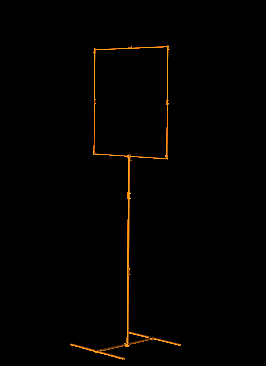
\includegraphics[height=9cm]{fig/gate}

			\end{minipage}
			\begin{minipage}{0.4\textwidth}
				\centering
				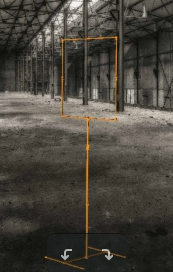
\includegraphics[height=9cm]{fig/gate_backgr}
				
			\end{minipage}
\caption{Example for Generated Sample}
		\end{figure}
	\end{block}

\end{column}



%%%% This is the THIRD column
\begin{column}{.45\textwidth}

	
	\begin{block}{Research Questions}
		
		\begin{enumerate}
			\item \textbf{How can we detect objects that consist mainly of background, namely the gates in an autonomous drone race?}
			\item \textbf{How can we deal with the limited amount of available training data?}
			\item \textbf{How can we deal with the limited computational resources on the MAV?}
		\end{enumerate}
		
		
	\end{block}
\begin{figure}
	
	\begin{minipage}{0.4\textwidth}
		\centering
		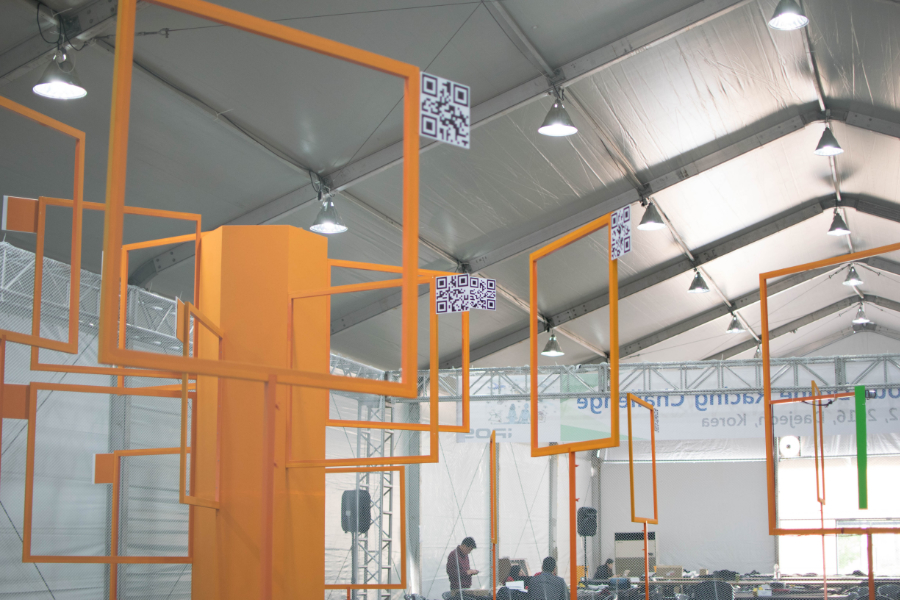
\includegraphics[height=9cm]{fig/iros-pic11}
		\caption{Race Court at IROS2011}
	\end{minipage}
	\begin{minipage}{0.4\textwidth}
		\centering
		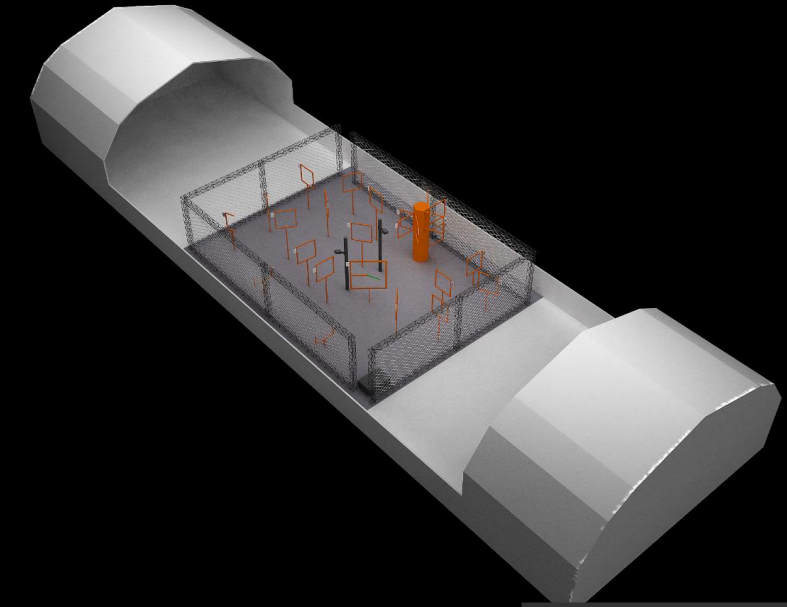
\includegraphics[height=9cm]{fig/court}
		\caption{3D Modell of Race Court}
	\end{minipage}
	\label{fig:angl-pr}
\end{figure}

\begin{figure}
	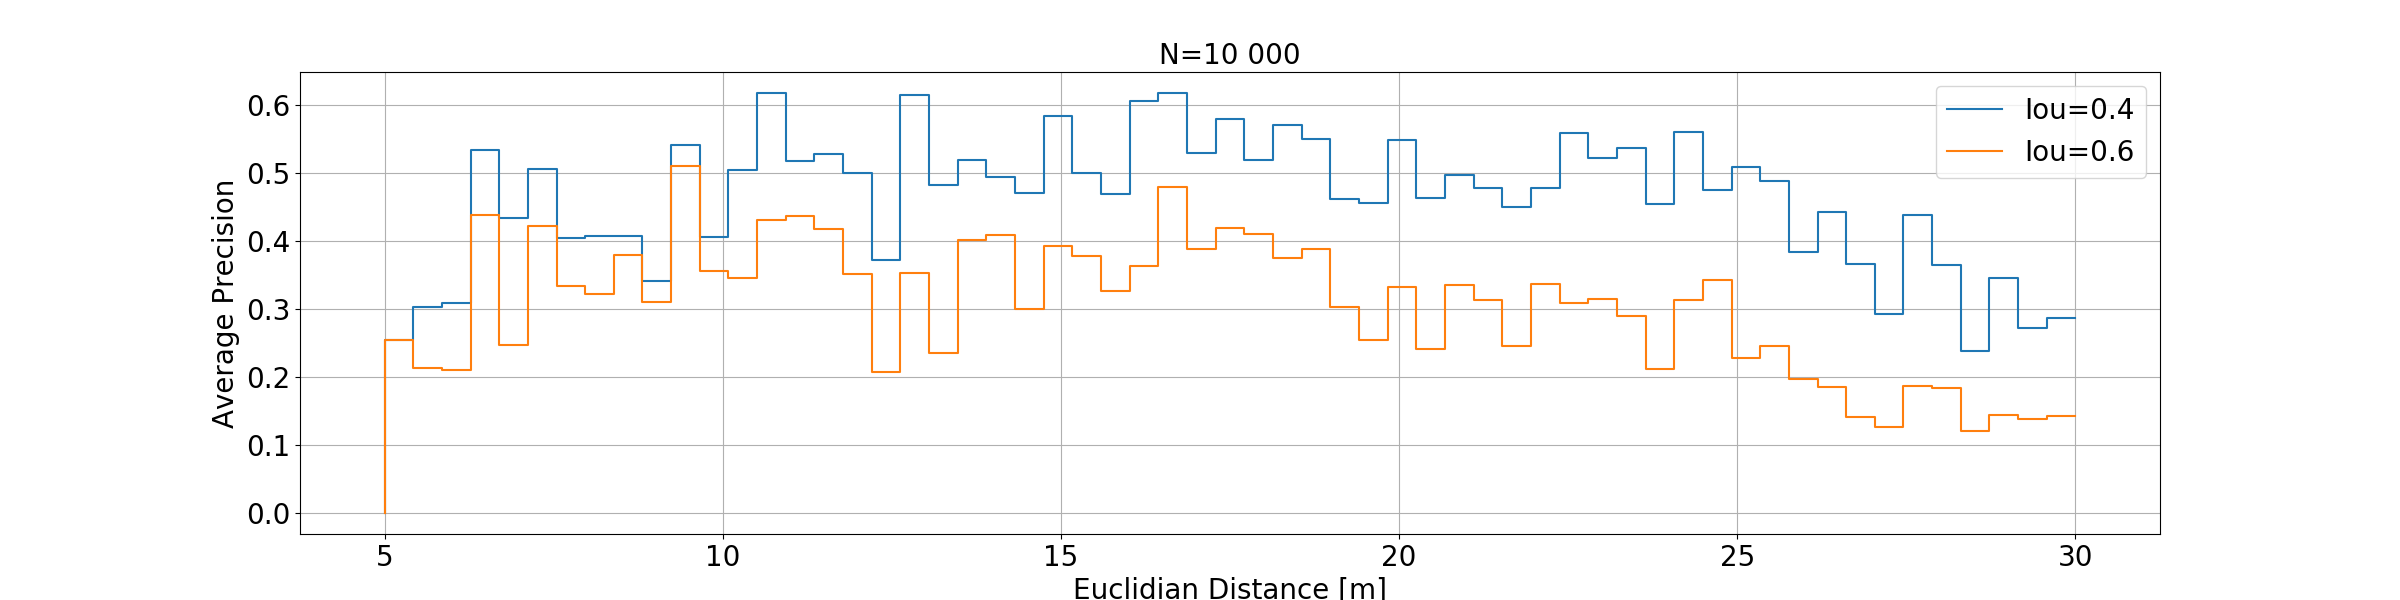
\includegraphics[width=\textwidth]{fig/meanAP-eucl}
	
	\label{fig:meanAP-eucl}
\end{figure}
\begin{figure}
	\centering
	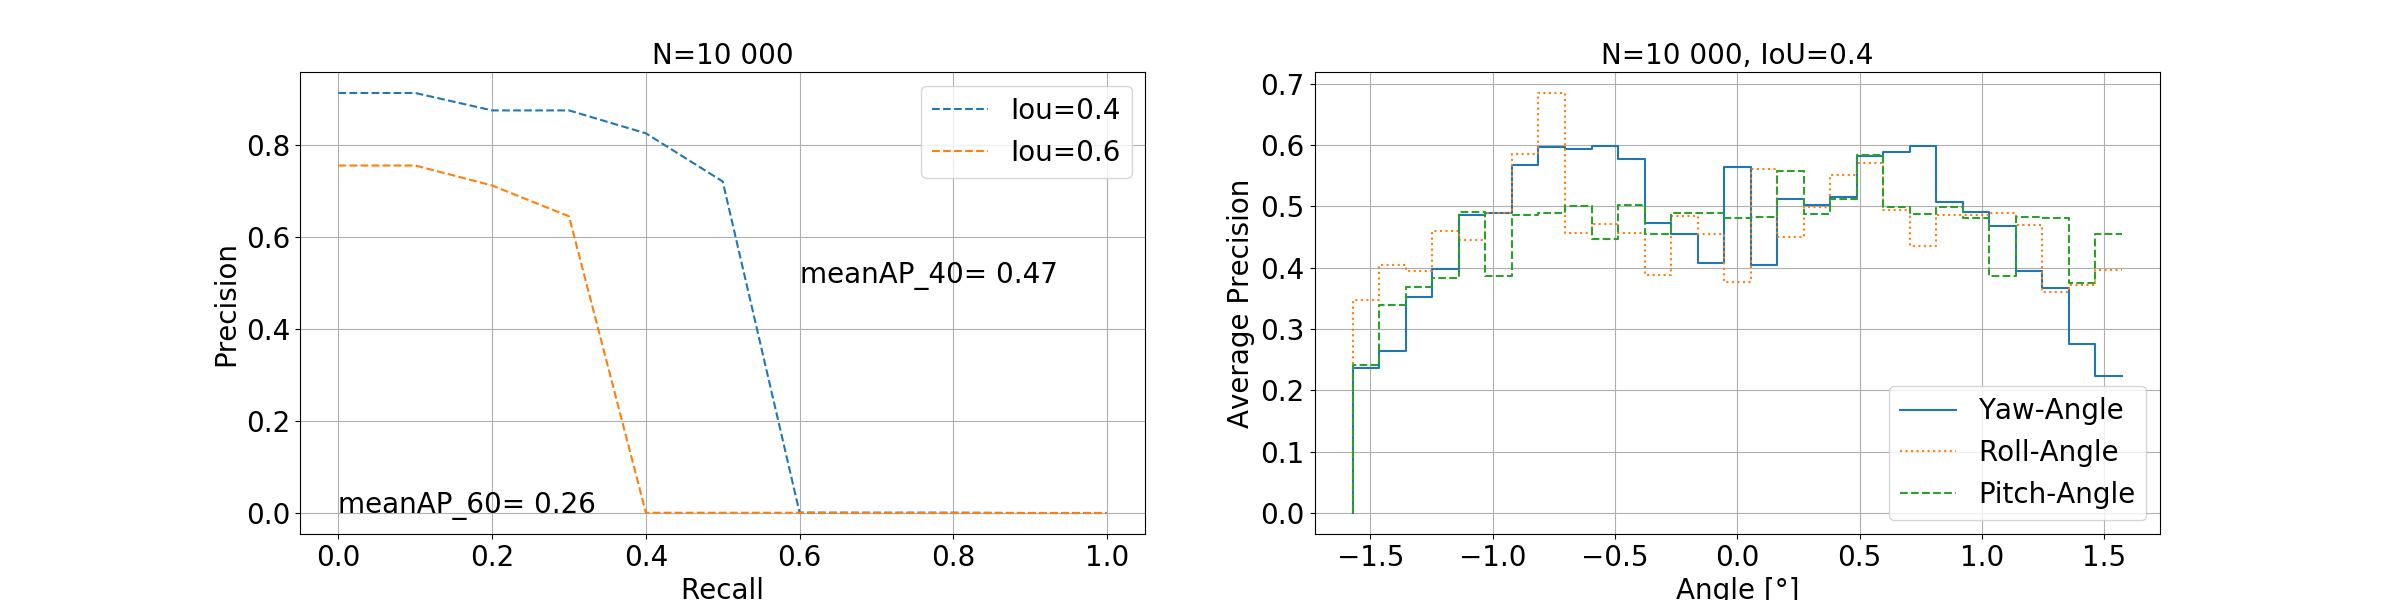
\includegraphics[width=\textwidth]{fig/angle-pr}
	
	\label{fig:angl-pr}
\end{figure}

	\begin{block}{Results}
		The results presented are evaluated on a generated dataset with 10 000 images. A detection is noted as correct if the intersection-over-union (IOU) between the predicted and the true bounding box exceeds a threshold. The average precision corresponds to the average precision over all recall levels. To evaluate the effects of the camera position results are grouped in bins of 0.5m / 6\degree. For each bin the average precision is calculated.
	\end{block}

%----------------------------------------------------------------------------------------
%   REFERENCES
%----------------------------------------------------------------------------------------





\end{column}
%%%% Second Column
\begin{column}{.25\textwidth}
	\begin{block}{Object Detectors}
		
		Object detection is a well-studies field in computer vision. Several benchmarks like the Pascal VOC challenge evaluate methods in terms of detection performance. For this thesis speed plays an important role. Methods with high detection performance that take several seconds to process on image can't be used on the MAV. To this end one model has been evaluated namely the "Yolo" - object detector \cite{Redmon}. Potential further methods are "SSD"\cite{Liu} or DPMs \cite{felzenszwalb2008discriminatively}. An example prediction for Yolo and SSD can be seen in Figure \ref{fig:ssd}.
		
		\begin{figure}
			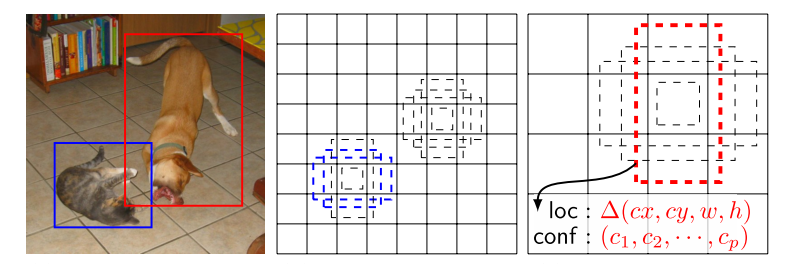
\includegraphics[height=6cm]{fig/ssd}
			\caption{Example SSD \cite{Liu}}
			\label{fig:ssd}
		\end{figure}	
		
	\end{block}


	
	\begin{block}{Conclusion}
		
		The overall meanAP of 47 \% with an IoU of 40\% can't be considered as decent result yet. However, this also contains results at positions that are out of the expected flight range. The results across precisions are quite inconsistent, one can see a slight deterioration in performance at higher and lower distances.
		
		Increasing the IoU threshold to 0.6 leads to heavy deterioration in performance. Hence, the bounding boxes are not that accurate yet. As this is crucial for the MAV navigation, improvement is required.
		

	\end{block}
	\begin{alertblock}{References}
		
		\nocite{*} % Insert publications even if they are not cited in the poster
		\small{\bibliographystyle{unsrt}
			\bibliography{sample}\vspace{0.75in}}
		
	\end{alertblock}
\end{column}


\end{columns}





\end{frame}
\end{document}